\subsection{Data model}
\label{sec:contribution:data}

\begin{figure*}[ht]
    \centering
    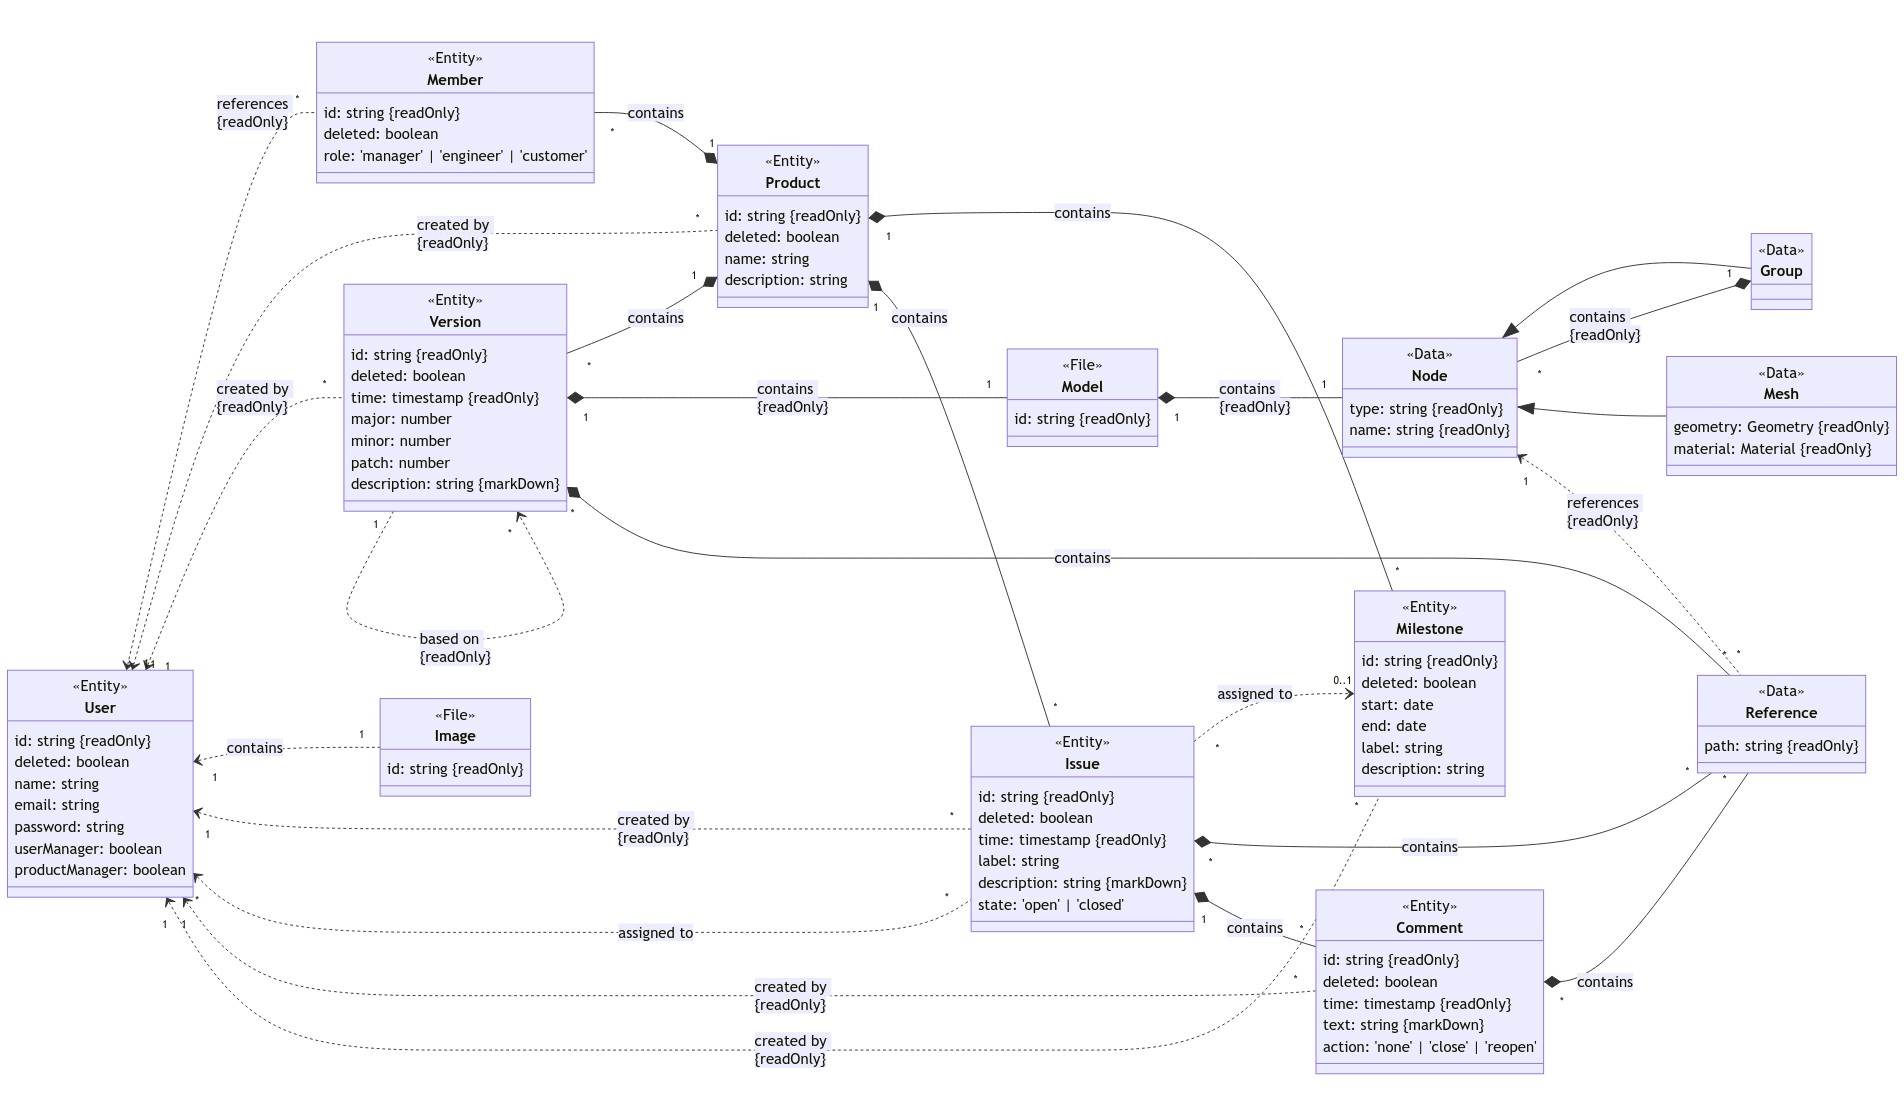
\includegraphics[width=\textwidth]{data-model.png}
    \caption{Integrated data model for improved information exchange between customers, project managers, requirements engineers, and product designers}
    \label{fig: datamodel}
\end{figure*}

This section describes the integrated data model as shown in Figure~\ref{fig: datamodel}.
The data model contains the following entities: \textit{User}, \textit{Product}, \textit{Version}, \textit{Issue}, \textit{Comment}, \textit{Milestone}, and \textit{Member}.
Note that all entities share a common identifier attribute, which is used for referencing and linking entities.
Furthermore, all entities share a common deleted attribute, which is used to hide entities after removal.

% User
The \textit{User} entity represents the individual stakeholders, who access the tool during product development.
The entity defines an email and a password attribute, which are used for authentication purposes.
Additionally, the entity defines a name attribute, which is used for a human-readable identification of stakeholders.
Similarly, the entity links an \textit{Image} file, which provides a human-interpretable visual representation of stakeholders (i.e.\ a profile picture).
Furthermore, the entity defines a user manager and a product manager flag, which are used for permission control as explained later.

% Product
The \textit{Product} entity represents the individual products or product development projects managed with the tool.
The entity is always linked to a \textit{User} entity, representing the stakeholder who created the product in the first place.
Then, the entity defines a name attribute, which is used to identify the product in a human-readable manner.
Furthermore, the entity defines a description attribute, which is used to explain the purpose of the product only briefly.

% Member
The \textit{Member} entity represents the permission to access certain product data through the tool.
Consequently, the entity is linked to a \textit{Product} entity, representing the product for which access is granted.
Also, the entity is linked to a \textit{User} entity, representing the stakeholder who is granted product access.
Finally, the entity defines a \textit{role} attribute, which controls the permission level as explained later, and which can have one of three values: \textit{manager}, \textit{engineer}, or \textit{customer}.

% Version
The \textit{Version} entity represents a revision of the product design created by a product designer.
The entity is linked to a \textit{Product} entity to identify the product, for which the design revision was created.
Similarly, the entity is linked to a \textit{User} entity to identify the product designer, who was responsible for creating the design revision.
Furthermore, the entity is linked to previous \textit{Version} entities to document the history of design revisions including version branching and merging.
Then, the entity defines a major, a minor, and a patch number, which together represent a version number according to semantic versioning\footnote{\url{https://semver.org/}} practices.
Also, the entity defined a description, which provides a human-readable explanation of the design changes that have been applied.
Finally, the entity links a \textit{Model} file, which represents the actual design data including assembly and part structures as well as geometry and material information.

% Model
We work with a generic representation of \textit{Model} files, which is independent of the CAD tool vendor and data format used.
We assume a model contains \textit{Node} objects, which carry all the engineering information created by the product designer.
Furthermore, we assume a node defines a name attribute, which can be used as for human-readable identification of nodes.
Additionally, we assume a node provides a type attribute, which can be used to distinguish different types of nodes.
At the moment, we distinguish two types of nodes, namely \textit{Group} nodes and \textit{Mesh} nodes.
Groups represent the assembly structures and provide links to child nodes being assembled, which can be both groups and meshes.
Meshes, on the other hand, represent the atomic parts of the product design such as screws or rivets, and carry geometry and material information.
Technically, we work with the glTF\footnote{\url{https://www.khronos.org/gltf/}} format for representing models including their node structures as well as their geometry and material information.
However, the STEP\footnote{\url{https://www.iso.org/standard/66654.html}} format or the COLLADA\footnote{\url{https://www.khronos.org/collada/}} format could be used equally well, since they follow the same principles.
In fact, even a vendor-specific data format could be used as long as appropriate parsers are available.

% Milestone
The \textit{Milestone} entity essentially represents project schedules including deadlines for the realization of design tasks.
The entity always links a \textit{Product} entity to identify the product or project the milestone belongs to.
Furthermore, the entity links a \textit{User} entity to identify the product manager, who created the milestone.
Finally, the entity defines a start and an end date, which represent the time frame for working on the milestone and achieving its goals.

% Issue
The \textit{Issue} entity represents design tasks, which have to be performed by product designers during product development projects.
The entity is always linked to a \textit{Product} entity to identify the product or project the issue belongs to.
Furthermore, the entity is linked to multiple \textit{User} entities to identify the one stakeholder, who reported the issue in the first place, and to identify the product designers, who are responsible for issue resolution.
Moreover, the entity can be linked to a \textit{Milestone} entity to identify the time frame, within which the issue should be resolved.
Then, the entity defines a time attribute, which records the point in time when the issue was reported originally.
Also, the entity defines a label attribute, which provides a human-readable summary of the issue.
Additionally, the entity defines a text attribute, which provides a more detailed explanation of the design task including Markdown-based\footnote{\url{https://www.Markdownguide.org/}} \textit{Reference} objects as explained later.
Finally, the entity defines a state attribute, which enables us to distinguish between open and closed design tasks.

% Comment
The \textit{Comment} entity represents discussions between stakeholders on issues or design tasks respectively.
The entity links an \textit{Issue} entity to identify the issue or design task the comment belongs to.
Furthermore, the entity links a \textit{User} entity to identify the stakeholder, who posted the comment.
Then, the entity defines a time attribute, which records the point in time when the comment was posted.
Additionally, the entity defines a text attribute, which contains the actual content of the comment including Markdown-based \textit{Reference} objects as explained later.
Finally, the entity defines an action attribute, which can be used to close or reopen an issue by posting a comment.

% Reference
As explained previously, we work with a Markdown-based representation of \textit{Reference} objects, which can be contained in the description of \textit{Issue} entities as well as \textit{Comment} entities.
These references can be used to refer to \textit{Node} objects, that are contained in the CAD models of design revisions for a particular product or project.
Consequently, the specification and discussion of design tasks can be enriched with links to assembly structures and parts, which have been designed and delivered previously.